\documentclass[twoside]{book}

% Packages required by doxygen
\usepackage{fixltx2e}
\usepackage{calc}
\usepackage{doxygen}
\usepackage{graphicx}
\usepackage[utf8]{inputenc}
\usepackage{makeidx}
\usepackage{multicol}
\usepackage{multirow}
\PassOptionsToPackage{warn}{textcomp}
\usepackage{textcomp}
\usepackage[nointegrals]{wasysym}
\usepackage[table]{xcolor}

% NLS support packages
\usepackage[french]{babel}

% Font selection
\usepackage[T1]{fontenc}
\usepackage{mathptmx}
\usepackage[scaled=.90]{helvet}
\usepackage{courier}
\usepackage{amssymb}
\usepackage{sectsty}
\renewcommand{\familydefault}{\sfdefault}
\allsectionsfont{%
  \fontseries{bc}\selectfont%
  \color{darkgray}%
}
\renewcommand{\DoxyLabelFont}{%
  \fontseries{bc}\selectfont%
  \color{darkgray}%
}
\newcommand{\+}{\discretionary{\mbox{\scriptsize$\hookleftarrow$}}{}{}}

% Page & text layout
\usepackage{geometry}
\geometry{%
  a4paper,%
  top=2.5cm,%
  bottom=2.5cm,%
  left=2.5cm,%
  right=2.5cm%
}
\tolerance=750
\hfuzz=15pt
\hbadness=750
\setlength{\emergencystretch}{15pt}
\setlength{\parindent}{0cm}
\setlength{\parskip}{0.2cm}
\makeatletter
\renewcommand{\paragraph}{%
  \@startsection{paragraph}{4}{0ex}{-1.0ex}{1.0ex}{%
    \normalfont\normalsize\bfseries\SS@parafont%
  }%
}
\renewcommand{\subparagraph}{%
  \@startsection{subparagraph}{5}{0ex}{-1.0ex}{1.0ex}{%
    \normalfont\normalsize\bfseries\SS@subparafont%
  }%
}
\makeatother

% Headers & footers
\usepackage{fancyhdr}
\pagestyle{fancyplain}
\fancyhead[LE]{\fancyplain{}{\bfseries\thepage}}
\fancyhead[CE]{\fancyplain{}{}}
\fancyhead[RE]{\fancyplain{}{\bfseries\leftmark}}
\fancyhead[LO]{\fancyplain{}{\bfseries\rightmark}}
\fancyhead[CO]{\fancyplain{}{}}
\fancyhead[RO]{\fancyplain{}{\bfseries\thepage}}
\fancyfoot[LE]{\fancyplain{}{}}
\fancyfoot[CE]{\fancyplain{}{}}
\fancyfoot[RE]{\fancyplain{}{\bfseries\scriptsize Généré le Mercredi 15 Octobre 2014 15\+:14\+:40 pour Grosmembre par Doxygen }}
\fancyfoot[LO]{\fancyplain{}{\bfseries\scriptsize Généré le Mercredi 15 Octobre 2014 15\+:14\+:40 pour Grosmembre par Doxygen }}
\fancyfoot[CO]{\fancyplain{}{}}
\fancyfoot[RO]{\fancyplain{}{}}
\renewcommand{\footrulewidth}{0.4pt}
\renewcommand{\chaptermark}[1]{%
  \markboth{#1}{}%
}
\renewcommand{\sectionmark}[1]{%
  \markright{\thesection\ #1}%
}

% Indices & bibliography
\usepackage{natbib}
\usepackage[titles]{tocloft}
\setcounter{tocdepth}{3}
\setcounter{secnumdepth}{5}
\makeindex

% Hyperlinks (required, but should be loaded last)
\usepackage{ifpdf}
\ifpdf
  \usepackage[pdftex,pagebackref=true]{hyperref}
\else
  \usepackage[ps2pdf,pagebackref=true]{hyperref}
\fi
\hypersetup{%
  colorlinks=true,%
  linkcolor=blue,%
  citecolor=blue,%
  unicode%
}

% Custom commands
\newcommand{\clearemptydoublepage}{%
  \newpage{\pagestyle{empty}\cleardoublepage}%
}


%===== C O N T E N T S =====

\begin{document}

% Titlepage & ToC
\hypersetup{pageanchor=false,
             bookmarks=true,
             bookmarksnumbered=true,
             pdfencoding=unicode
            }
\pagenumbering{roman}
\begin{titlepage}
\vspace*{7cm}
\begin{center}%
{\Large Grosmembre \\[1ex]\large 0.\+1 }\\
\vspace*{1cm}
{\large Généré par Doxygen 1.8.8}\\
\vspace*{0.5cm}
{\small Mercredi 15 Octobre 2014 15:14:40}\\
\end{center}
\end{titlepage}
\clearemptydoublepage
\tableofcontents
\clearemptydoublepage
\pagenumbering{arabic}
\hypersetup{pageanchor=true}

%--- Begin generated contents ---
\chapter{Cahier des charges}
\label{md_cahier_des_charges}
\hypertarget{md_cahier_des_charges}{}
\input{md_cahier_des_charges}
\chapter{Index hiérarchique}
\section{Hiérarchie des classes}
Cette liste d'héritage est classée approximativement par ordre alphabétique \+:\begin{DoxyCompactList}
\item Q\+Widget\begin{DoxyCompactList}
\item \contentsline{section}{Widget}{\pageref{class_widget}}{}
\end{DoxyCompactList}
\end{DoxyCompactList}

\chapter{Index des classes}
\section{Liste des classes}
Liste des classes, structures, unions et interfaces avec une brève description \+:\begin{DoxyCompactList}
\item\contentsline{section}{\hyperlink{class_widget}{Widget} }{\pageref{class_widget}}{}
\end{DoxyCompactList}

\chapter{Documentation des classes}
\hypertarget{class_widget}{\section{Référence de la classe Widget}
\label{class_widget}\index{Widget@{Widget}}
}
Graphe d'héritage de Widget\+:\begin{figure}[H]
\begin{center}
\leavevmode
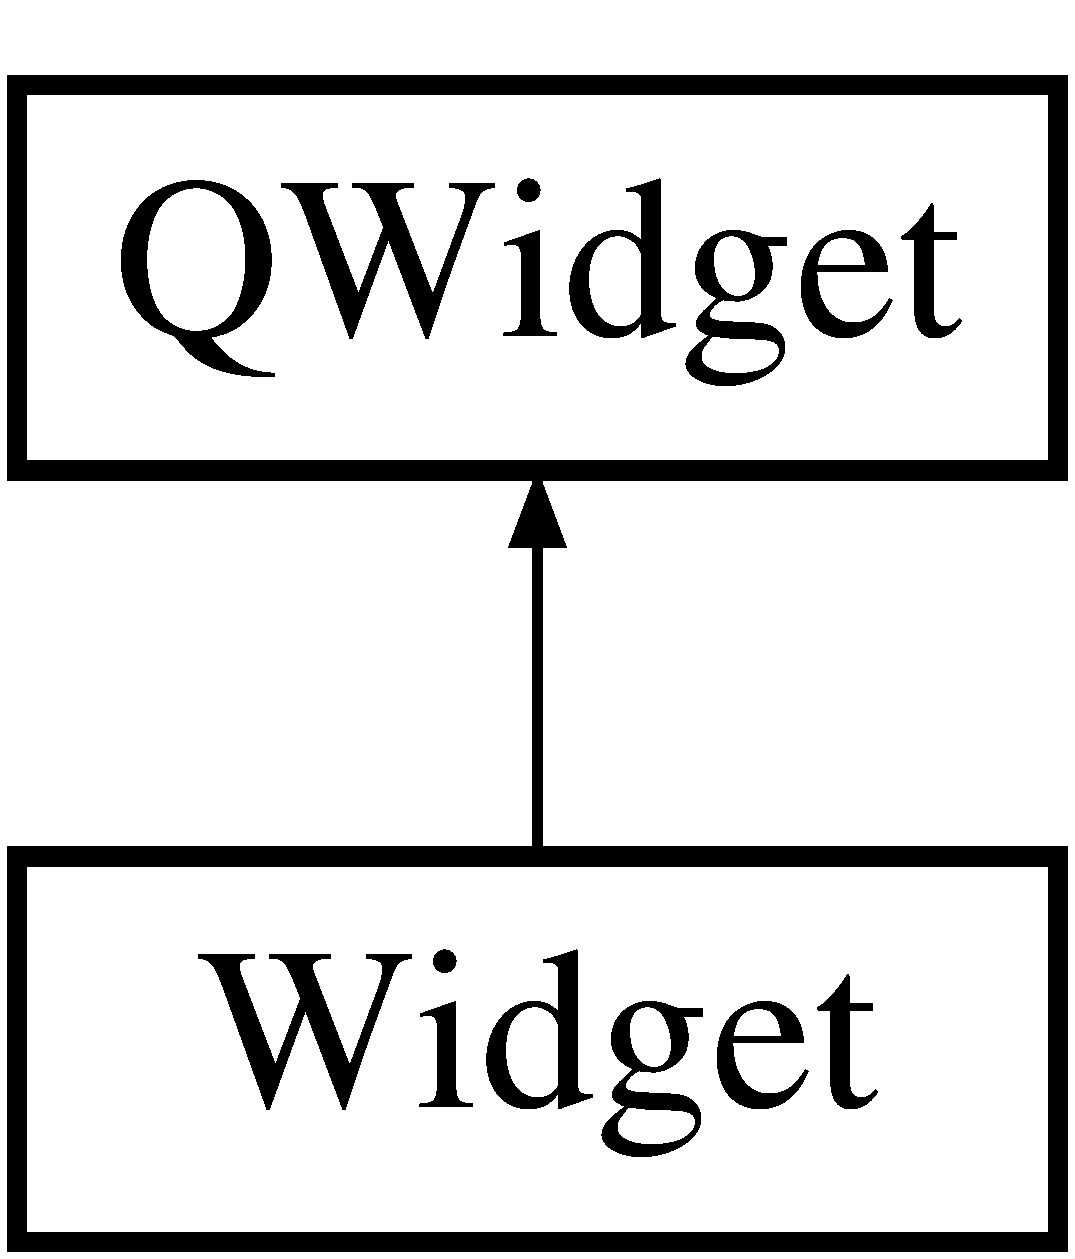
\includegraphics[height=2.000000cm]{class_widget}
\end{center}
\end{figure}
\subsection*{Connecteurs publics}
\begin{DoxyCompactItemize}
\item 
void \hyperlink{class_widget_a305d97da24c5634217d536c04a05dc9f}{set\+Mail} (Q\+String s)
\begin{DoxyCompactList}\small\item\em \hyperlink{class_widget_a305d97da24c5634217d536c04a05dc9f}{Widget\+::set\+Mail} remplit le champ m\+\_\+mail (adresse mail) à partir du pattern '\href{mailto:prenom.nom@etu.univ-nantes.fr}{\tt prenom.\+nom@etu.\+univ-\/nantes.\+fr}. \end{DoxyCompactList}\item 
\hypertarget{class_widget_aa2cdb764abf57ef228bce94aa98283cd}{void {\bfseries flush} ()}\label{class_widget_aa2cdb764abf57ef228bce94aa98283cd}

\item 
\hypertarget{class_widget_a6ba5b00519d83cee3d4f744e7d2a61aa}{void {\bfseries add\+Member} ()}\label{class_widget_a6ba5b00519d83cee3d4f744e7d2a61aa}

\item 
\hypertarget{class_widget_a05e84745aa8a84f5dc93b1926adb9d09}{void {\bfseries list\+Member} ()}\label{class_widget_a05e84745aa8a84f5dc93b1926adb9d09}

\item 
\hypertarget{class_widget_a1e98071dfb4cd77ec3c6af2366ba9346}{void {\bfseries updatelist\+Member} ()}\label{class_widget_a1e98071dfb4cd77ec3c6af2366ba9346}

\end{DoxyCompactItemize}
\subsection*{Fonctions membres publiques}
\begin{DoxyCompactItemize}
\item 
\hyperlink{class_widget_a29531c7f141e461322981b3b579d4590}{Widget} (Q\+Widget $\ast$parent=0)
\begin{DoxyCompactList}\small\item\em \hyperlink{class_widget_a29531c7f141e461322981b3b579d4590}{Widget\+::\+Widget} widget principal. \end{DoxyCompactList}\item 
\hypertarget{class_widget_a5020ae4d7597c3a4992b1b4f29682029}{bool {\bfseries est\+Dedans} (Q\+String nom, Q\+String prenom, Q\+String num\+Etu)}\label{class_widget_a5020ae4d7597c3a4992b1b4f29682029}

\item 
\hypertarget{class_widget_aa24f66bcbaaec6d458b0980e8c8eae65}{\hyperlink{class_widget_aa24f66bcbaaec6d458b0980e8c8eae65}{$\sim$\+Widget} ()}\label{class_widget_aa24f66bcbaaec6d458b0980e8c8eae65}

\begin{DoxyCompactList}\small\item\em \hyperlink{class_widget_aa24f66bcbaaec6d458b0980e8c8eae65}{Widget\+::$\sim$\+Widget} un destructeur. \end{DoxyCompactList}\end{DoxyCompactItemize}


\subsection{Documentation des constructeurs et destructeur}
\hypertarget{class_widget_a29531c7f141e461322981b3b579d4590}{\index{Widget@{Widget}!Widget@{Widget}}
\index{Widget@{Widget}!Widget@{Widget}}
\subsubsection[{Widget}]{\setlength{\rightskip}{0pt plus 5cm}Widget\+::\+Widget (
\begin{DoxyParamCaption}
\item[{Q\+Widget $\ast$}]{parent = {\ttfamily 0}}
\end{DoxyParamCaption}
)}}\label{class_widget_a29531c7f141e461322981b3b579d4590}


\hyperlink{class_widget_a29531c7f141e461322981b3b579d4590}{Widget\+::\+Widget} widget principal. 


\begin{DoxyParams}{Paramètres}
{\em parent} & prend en paramètre le \hyperlink{class_widget}{Widget} parent de classe Q\+Widget \\
\hline
\end{DoxyParams}
s\+\_\+list Liste des attributs renseignés lors de l’inscription d’un membre \+: 

\subsection{Documentation des fonctions membres}
\hypertarget{class_widget_a305d97da24c5634217d536c04a05dc9f}{\index{Widget@{Widget}!set\+Mail@{set\+Mail}}
\index{set\+Mail@{set\+Mail}!Widget@{Widget}}
\subsubsection[{set\+Mail}]{\setlength{\rightskip}{0pt plus 5cm}void Widget\+::set\+Mail (
\begin{DoxyParamCaption}
\item[{Q\+String}]{s}
\end{DoxyParamCaption}
)\hspace{0.3cm}{\ttfamily [slot]}}}\label{class_widget_a305d97da24c5634217d536c04a05dc9f}


\hyperlink{class_widget_a305d97da24c5634217d536c04a05dc9f}{Widget\+::set\+Mail} remplit le champ m\+\_\+mail (adresse mail) à partir du pattern '\href{mailto:prenom.nom@etu.univ-nantes.fr}{\tt prenom.\+nom@etu.\+univ-\/nantes.\+fr}. 


\begin{DoxyParams}{Paramètres}
{\em s} & de type Q\+String \\
\hline
\end{DoxyParams}


La documentation de cette classe a été générée à partir des fichiers suivants \+:\begin{DoxyCompactItemize}
\item 
widget.\+h\item 
widget.\+cpp\end{DoxyCompactItemize}

%--- End generated contents ---

% Index
\newpage
\phantomsection
\addcontentsline{toc}{chapter}{Index}
\printindex

\end{document}
